\graphicspath{{Introduccion/Figs/}}

\setcounter{chapter}{1}
\chapter*{Introducción} 
\addcontentsline{toc}{chapter}{Introducción}
\setcounter{figure}{0}
\setcounter{table}{0}
\setcounter{section}{0}

\section{Silenciamiento génico y ARN pequeños en plantas}

El control de la expresión génica es un proceso vital para los organismos unicelulares.
Este proceso es utilizado por las células para ajustar la expresión génica durante el desarrollo o frente a los cambios en su ambiente.
En plantas, la generación de los numerosos tipos celulares diferentes que forman en conjunto un organismo multicelular depende de que los genes se activen en las células adecuadas y en los momentos precisos del desarrollo.
Muchos de los mecanismos regulatorios operan a nivel genético generando un control a nivel transcripcional y post-transcripcional.

En los últimos años se ha descubierto que pequeñas moléculas de 20 a 25 nucleótidos de longitud, son reguladores críticos de la expresión génica en eucariotas.
En plantas existen distintos tipos de ARN pequeños que, por diferencias en su biogénesis y modos de acción, han sido clasificados en distintas clases, aunque pueden compartir algunos elementos comunes.

\subsection{Variedades de ARN pequeños en plantas}
Los ARN pequeños provienen del procesamiento de regiones helicoidales de precursores de ARN.
Los mismos se pueden clasificar en dos grupos principales. 
Los derivados de precursores de doble hebra (ARNdh) formados por hibridación intermolecular de dos cadenas de ARN complementarias y los derivados de precursores de RNA de una sola hebra (ARNsh) que forman una estructura de tallo-burbuja.

Los ARN pequeños más abundantes, derivados de precursores de ARNdh, son conocidos como siARNs (del inglés small interfering RNAs). 
Éstos pueden ser de origen endógeno o exógeno.
A su vez, los siARNs se pueden clasificar en dos grupos, aquellos que producen un silenciamiento a nivel transcripcional (TGS, del inglés: Transcriptional Gene Silencing) \citep{pmid17943195, Voinnet2009669} y aquellos que lo producen a nivel post-transcripcional (PTGS, del inglés: Post Transcriptional Gene Silencing)\citep{pmid10542148}.

El primer grupo se origina a partir de ciertas regiones genómicas como transposones u otras secuencias repetitivas que son transcriptos por la ARN polimerasa IV.
Estos ARNsh se convierten en ARNdh por acción de una enzima ARN polimerasa dependiente de ARN llamada RDR2 (del inglés RNA-DEPENDENT RNA POLYMERASE2). 
A continuación los ARNdh son procesados por por una ribonuclease llamada DCL3 (del inglés DICER-LIKE3) que corta el ARNdh para liberar siARNs de 24 nt de longitud.
El segundo grupo, los PTGS son originados a partir de ARNs de virus o ARNm proveniente de un transgén. 
Estos ARNs se convierten en ARNdh por acción de RDR6 y el ARNdh resultante es procesado por DCL2 o DCL4 para finalmente librer siARN de 21-22 nt que serán encargados del silenciamiento post-transcripcional \citep{pmid18358247}.
Los roles biológicos del silenciamiento mediado por siARNs incluyen resistencia contra virus \citep{pmid11485817}, protección del genoma contra elementos móviles de ADN y roles regulatorios sobre genes endógenos \citep{pmid15372043, pmid17943195, Voinnet2009669}.

Existen otros ARNdh menos abundantes que han sido descubiertos posteriormente.
Este grupo está constituido por un lado por los ta-siARN (del inglés, trans-acting siRNAs) y por el otro lado los nat-siARNs y nat-miARNs (del inglés, natural antisense siRNAs y miRNAs) \citep{pmid17943195, pmid18501663, pmid16600909,Voinnet2009669}.

Los genes que darán lugar a ta-siARNs son transcriptos para dar lugar a un ARN no codificante denominados TAS.
Este transcripto luego es identificado y cortado por acción de un miARN que posee una secuencia complementaria al mismo \citep{Allen2005207}.
Los fragmentos de corte de un TAS se estabilizan y por la acción de RDR6, y se convierten en un ARNdh que es procesado por DCL4, generando ARNs pequeños de 21 nucleótidos.
Finalmente, algunos ta-siARNs se incorporan a un complejo RISC y guían el corte de los transcriptos de otros genes de manera similar a la acción de un miARN \citep{Allen2005207,pmid16040244,pmid16131612,Xie2005a}.

En contraste con los otros tipos de siARNs, que dependen de un RDR para sintetizar el precursor ARNdh, se cree que los precursores de ARNdh de NAT-siARNs (siARNs asociados a ARNs antisentido naturales, del inglés "Natural Antisens Transcripts") \citep{pmid16377568,pmid17071740}.
En este caso, dos ARNs independientes pueden ser complementarios debido a que fueron transcriptos por hebras opuestas en el mismo locus, y se denominan cis-NAT-siARNs. 
El ARNdh formado es procesado por DCL1 o DCL2 liberando siARNs primarios que inducen el corte sobre el ARNm expresado constitutivamente.
Posteriormente, una RDR sintetiza la hebra complementaria del ARNm cortado. 
Esto da lugar nuevamente a un ARNdh el cual es procesado por DCL1 para producir una sucesión de siARN ubicados en fase de 21 nt cada uno denominados nat-siARN secundarios \citep{pmid16377568,pmid17071740}.

Como contraste con los siARNs descriptos anteriormente, que son procesados por ARNdh, existe la posibilidad de que un ARN se pliegue sobre si mismo, formando un tallo y una burbuja (en inglés, "stem loop").
La clase más abundante de ARN pequeños derivados de precursores de ARNsh (ARN simple hebra) son los miARNs.
Tienen entre 20 y 22 nt de longitud y son originados de largos precursores con extensa estructura secundaria en forma tallo-burbuja.
Estos precursores luego son procesados por acción de DCL1, liberando el ARN maduro. 
Actúan como reguladores negativos de la expresión génica reprimiendo la expresión de genes endógenos principalmente a nivel post-transcripcional.
Esta regulación se puede dar a través de la inhibición de la traducción o del corte de los ARN mensajeros.
Tanto en animales como en plantas, existen un gran número de miARNs conservados en distintas especies.
En animales se han encontrado miARNs conservados en especies muy distantes como gusanos hasta humanos \citep{pmid11081512}.
Y en plantas sucede lo mismo, donde existen miARNs conservados desde musgos hasta dicotiledóneas \citep{pmid15849273,Axtell2008343,citeulike:8816489} (Figura \ref{fig:familias_miRNAs_conservados}).
No se han encontrado miARNs conservados en animales y en plantas, lo que sugiere que han aparecido en forma independientes durante la evolución \citep{citeulike:8816489}.
Si bien los miARNs en plantas y en animales comparten componentes básicos, su biogénesis y su modo de acción difiere entre ellos.


\begin{figure}[htbp!] 
    \centering    
    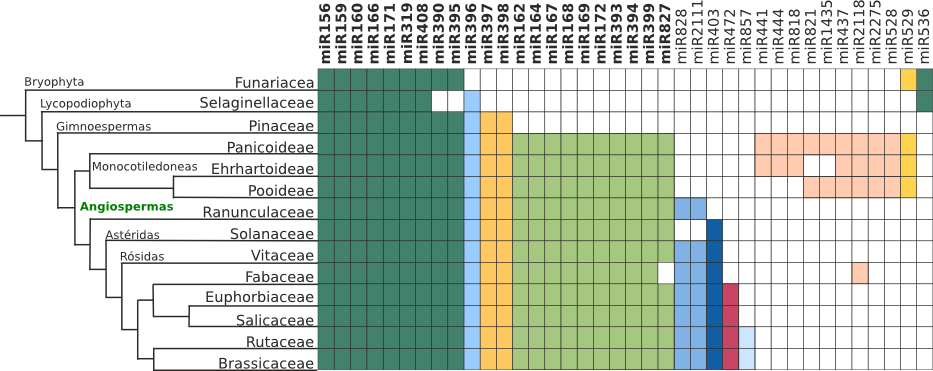
\includegraphics[width=1\textwidth]{familias_miRNAs_conservados.png}
    \caption[Familias de miARNs conservados en plantas]{
    \textbf{Familias de miARNs conservados en plantas.}
    Se muestran las familias de miARNs (columnas) y para cada una de ella se muestra en qué especies están conservadas (filas).
    En diferentes colores se muestra el rango de especies en el que se encuentran conservadas, para distintos grupos de familias.
    En negrita se marcan las familias conservadas en angiospermas. 
    MiR319 y miR159 que codifican para miARNs similares, fueron considerados como familias diferentes ya que regulan a genes blanco distintos \citep{Palatnik2007}.
    Adaptado de \citep{citeulike:8816489}.
    }
    \label{fig:familias_miRNAs_conservados}
\end{figure}

\section{miARNs en plantas}

Los miARNs son generados a partir de loci endógenos, tanto en animales como en plantas. 
Estos ARN pequeños controlan una gran variedad de procesos biológicos, como el desarrollo, la diferenciación y proliferación celular, y respuesta a estrés \citep{Voinnet2009669,pmid25118717,citeulike:8816489,pmid12869753,Axtell2008}

Hasta hoy, en \textit{A. thaliana} se han identificado más de 300 \citep{Kozomara2014} miARNs.
Se han utilizado distintos enfoques para identificar los miARNs: el clonado directo de ARN pequeños, secuenciación de alto rendimiento, estudios genéticos y predicciones bioinformáticas \citep{citeulike:8816489}, siendo esta última la más común para la mayoría de las especies.

Los miARNs en plantas están codificados por familias de genes de 1 a 32 miembros que dan lugar a miARNs maduros idénticos o muy similares.
Hasta el momento han sido definidas unas 42 familias de miARNs en plantas, las que regulan una amplia variedad de procesos biológicos.
Doce de dichas familias tienen como blanco ARN mensajeros que codifican factores de transcripción involucrados en el desarrollo, mientras que otras están relacionadas con rutas de respuesta a señales ambientales y hormonales, entre otros, estando la mayoría de ellas conservadas entre mono y dicotiledóneas \citep{Jones-Rhoades2006}.
Muchos de estos pequeños ARNs han aparecido recientemente en la evolución y por lo tanto aparecen en un número pequeño de especies \citep{Axtell2008,Axtell2008343}.
Además, no está claro si estos últimos tienen algún rol biológico \citep{Axtell2008343,citeulike:8816489}.

Sin embargo, existen 22 familias de miARNs que están altamente conservadas en las plantas, estando presentes en angiospermas, gimnospermas y algunas de ellas aún en plantas basales como los musgos \citep{Axtell2008,Arazi2005,pmid16623887} (Figura \ref{fig:familias_miRNAs_conservados}).
Muchas de estas familias de miARNs conservados cumplen funciones esenciales para la biología de las plantas \citep{Jones-Rhoades2006}.


\section{Biogénesis de miARNs}

\subsection{Procesamiento de miARNs en animales}

En animales, el procesamiento de los precursores es realizado en el núcleo y el citoplasma.
Luego de la transcripción, el complejo formado por la ribonucleasa de tipo III, DROSHA, y la proteína DiGeorge syndrome critical region gene 8 (DGCR8) produce un primer corte sobre el pri-miARN para liberar una estructura de tallo y burbuja denominado pre-miARN (Figura \ref{fig:procesamiento_animales}) \citep{pmid15531879, pmid15531877, pmid15574589, pmid15932881}.

A continuación, el pre-miARN es traslocado desde el núcleo hacia el citoplasma por la proteína de transporte nuclear EXPORTIN-5 (EXP5) \citep{pmid14631048,pmid14681208}.
En el citoplasma DICER conjuntamente con TRPB, otra proteína de unión a ARNdh, produce un segundo corte sobre el precursor para que liberar el dúplex miARN/miARN*.
Este segundo corte ocurre a $\sim$21 nt de distancia del sitio donde se había producido el primer corte por DROSHA.
Finalmente, el miARN maduro es incorporado al complejo RISC \citep{pmid19165215} (Figura \ref{fig:procesamiento_animales}).

Además de esta ruta canónica de procesamiento, recientemente se han descripto vías alternativas.
Para algunos precursores, el requerimiento de DROSHA puede ser suplantado por la maquinaria de corte y empalme (splicing) \citep{pmid17599402,pmid17589500}.
En el caso de otros, es necesaria la interacción de proteínas específicas con el loop terminal \citep{pmid17558416,pmid19458619}.
Por último, existen casos en donde, el procesamiento de ciertos precursores puede estar específicamente inhibido en ciertos tejidos o determinadas condiciones \citep{pmid18951094,pmid16738409,pmid18292307}.

\begin{figure}[htbp!] 
    \centering    
    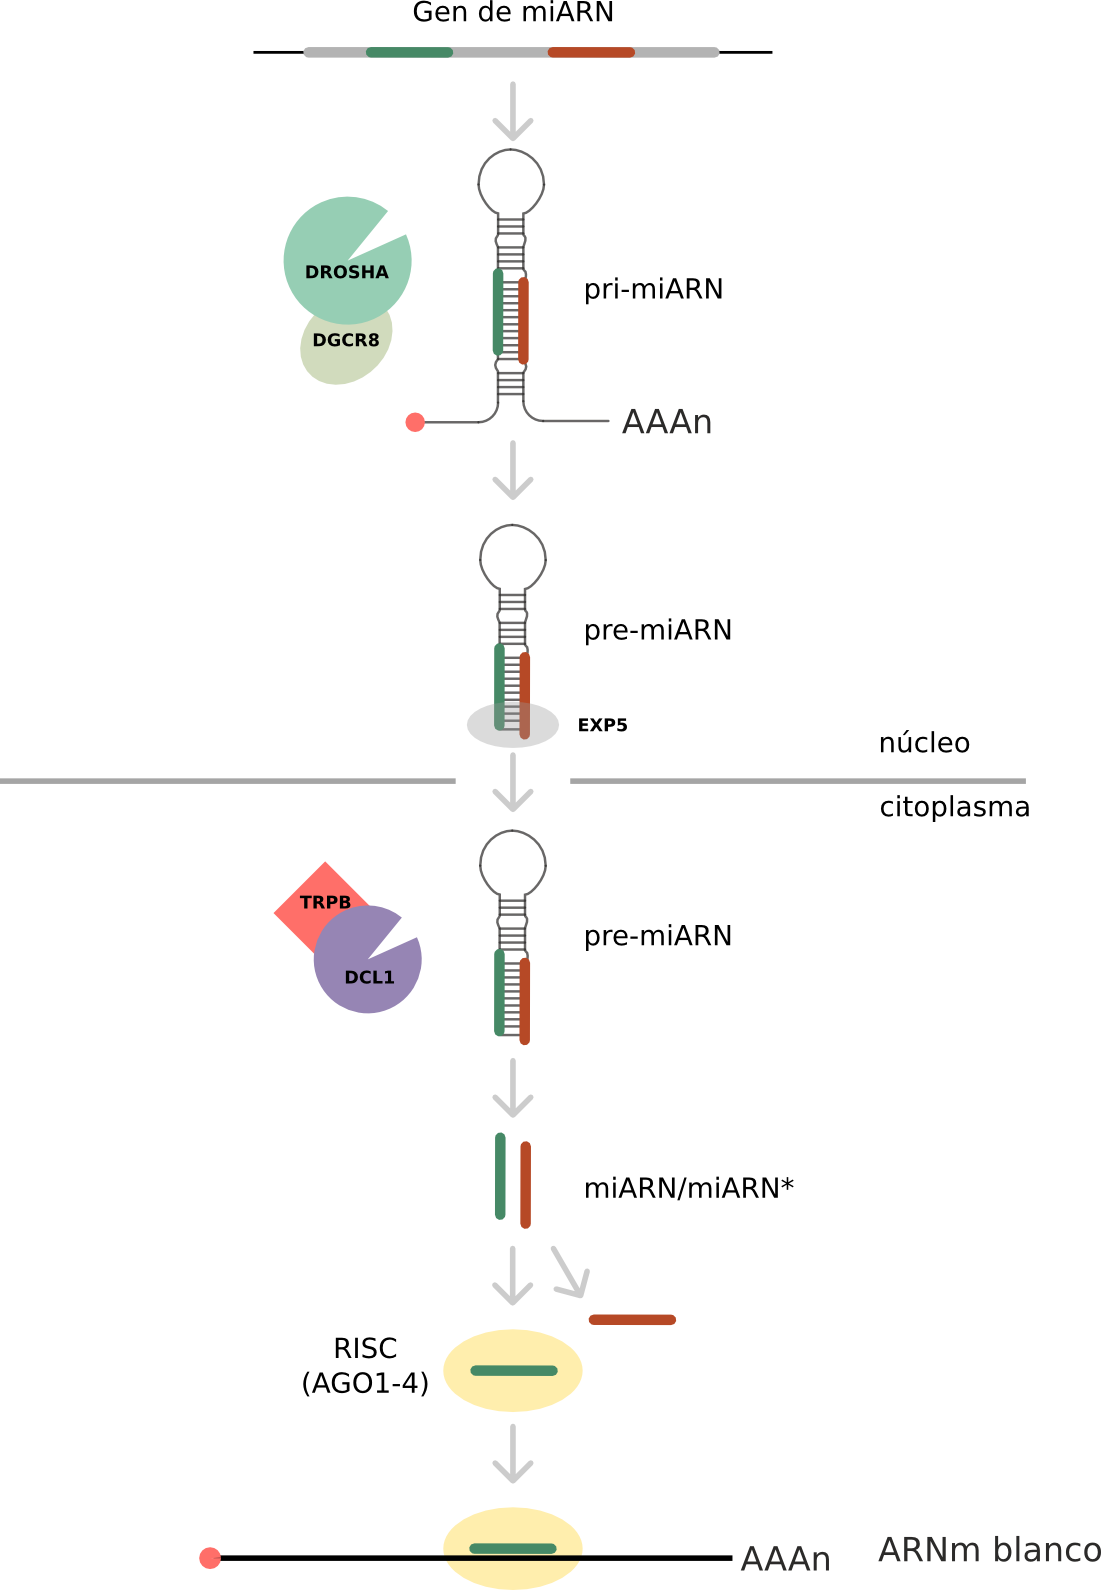
\includegraphics[width=.9\textwidth]{procesamiento_animales.png}
    \caption[Biogénesis de miARNs en animales]{
    \textbf{Mecanismo de procesamiento de miARNs en animales.}

    }
    \label{fig:procesamiento_animales}
\end{figure}


\subsection{Procesamiento de miARNs en plantas}

Los miARNs se diferencian de otros ARNs pequeños por su particular biogénesis que implica su escisión de un precursor con extensa estructura secundaria localizado en un largo transcripto primario (Figura \ref{fig:biogenesis_accion}).
En general, la biogénesis de estos ARN pequeños comienza con la transcripción por la ARN polimerasa II \citep{Xie2005a} a partir de unidades transcripcionales propias distribuidas en el genoma \citep{Reinhart2002}.
Los transcriptos primarios, llamados pri-miARNs, pueden tener varias kilobases de longitud y sufrir modificaciones post-transcripcionales como ser splicing, capping y poliadenilación. 
Estos transcriptos contienen precursores para miARNs con extensa estructura secundaria en forma de tallo-burbuja (stem-loop) \citep{Jones-Rhoades2006} (Figura \ref{fig:biogenesis_accion}).

En animales, el procesamiento comienza en el núcleo por DROSHA y finaliza en el citoplasma por la acción de DICER.
En plantas no existe un homólogo de DROSHA.
Los precursores son procesados completamente en el núcleo a través de la acción de una ribonucleasa llamada DCL1 \citep{Reinhart2002,pmid12417148} (del inglés DICER LIKE 1) en asociación con el cofactor proteico de unión a ARN de doble hebra HYL1 \citep{Han2004} (del inglés HYPONASTIC LEAVES 1) y la proteína SERRATE \citep{Lobbes2006} (Figura \ref{fig:biogenesis_accion}).

Al parecer es la estructura secundaria por sobre la secuencia primaria del precursor la más importante en la determinación del correcto procesamiento del mismo \citep{Bologna11112012} .
El producto generado a partir de los cortes llevados a cabo por DCL1, es un dúplex miARN-miARN* que luego continúa siendo procesado por otros componentes enzimáticos hasta dar lugar al miARN maduro de 21 nt.

El paso final de la biogénesis de los miARN es la incorporación asimétrica, a partir del dúplex miARN-miARN*, del miARN maduro dentro de un complejo de silenciamiento.
Este complejo se denomina RISC (del inglés RNAi Silencing Complex).
El componente central de todos los complejos de silenciamiento es un miembro de la familia de proteínas ARGONAUTA (AGO).
En Arabidopsis existen distintas proteínas AGO que participan en diferentes procesos biológicos \citep{Cellulaire2008} y la incorporación de los ARN pequeños en los distintos complejos depende de la identidad del nucleótido del extremo 5' y de la vía de biogénesis \citep{pmid18342361,Montgomery2008,Takeda2008} (Figura \ref{fig:biogenesis_accion}). 

En la mayoría de los miARNs el nucléotido extremo 5' es una U y en general la principal efectora de la actividad es AGO1 \citep{Voinnet2009669,pmid18342361,Vazquez2004a}.
Complejos RISC similares se encuentran presentes en células animales.
Más recientemente han sido identificadas proteínas adicionales que regularían la actividad de la maquinaria de procesamiento \citep{Bologna11112012}.

En animales, los miARNs reconocen principalmente sitios blancos ubicados en la región 3' no codificante de ARN mensajeros blanco inhibiendo su traducción.
En cambio en plantas, es más común que los miARNs se unan a secuencias complementarias que se localizan dentro los ARNm blanco en la región codificante señalándolos para su degradación \citep{Jones-Rhoades2006}.
En cualquier caso, es el miARN el que proporciona la especificidad contra las moléculas de ARN blanco \citep{Bartel2004}.

\begin{figure}[htbp!] 
    \centering    
    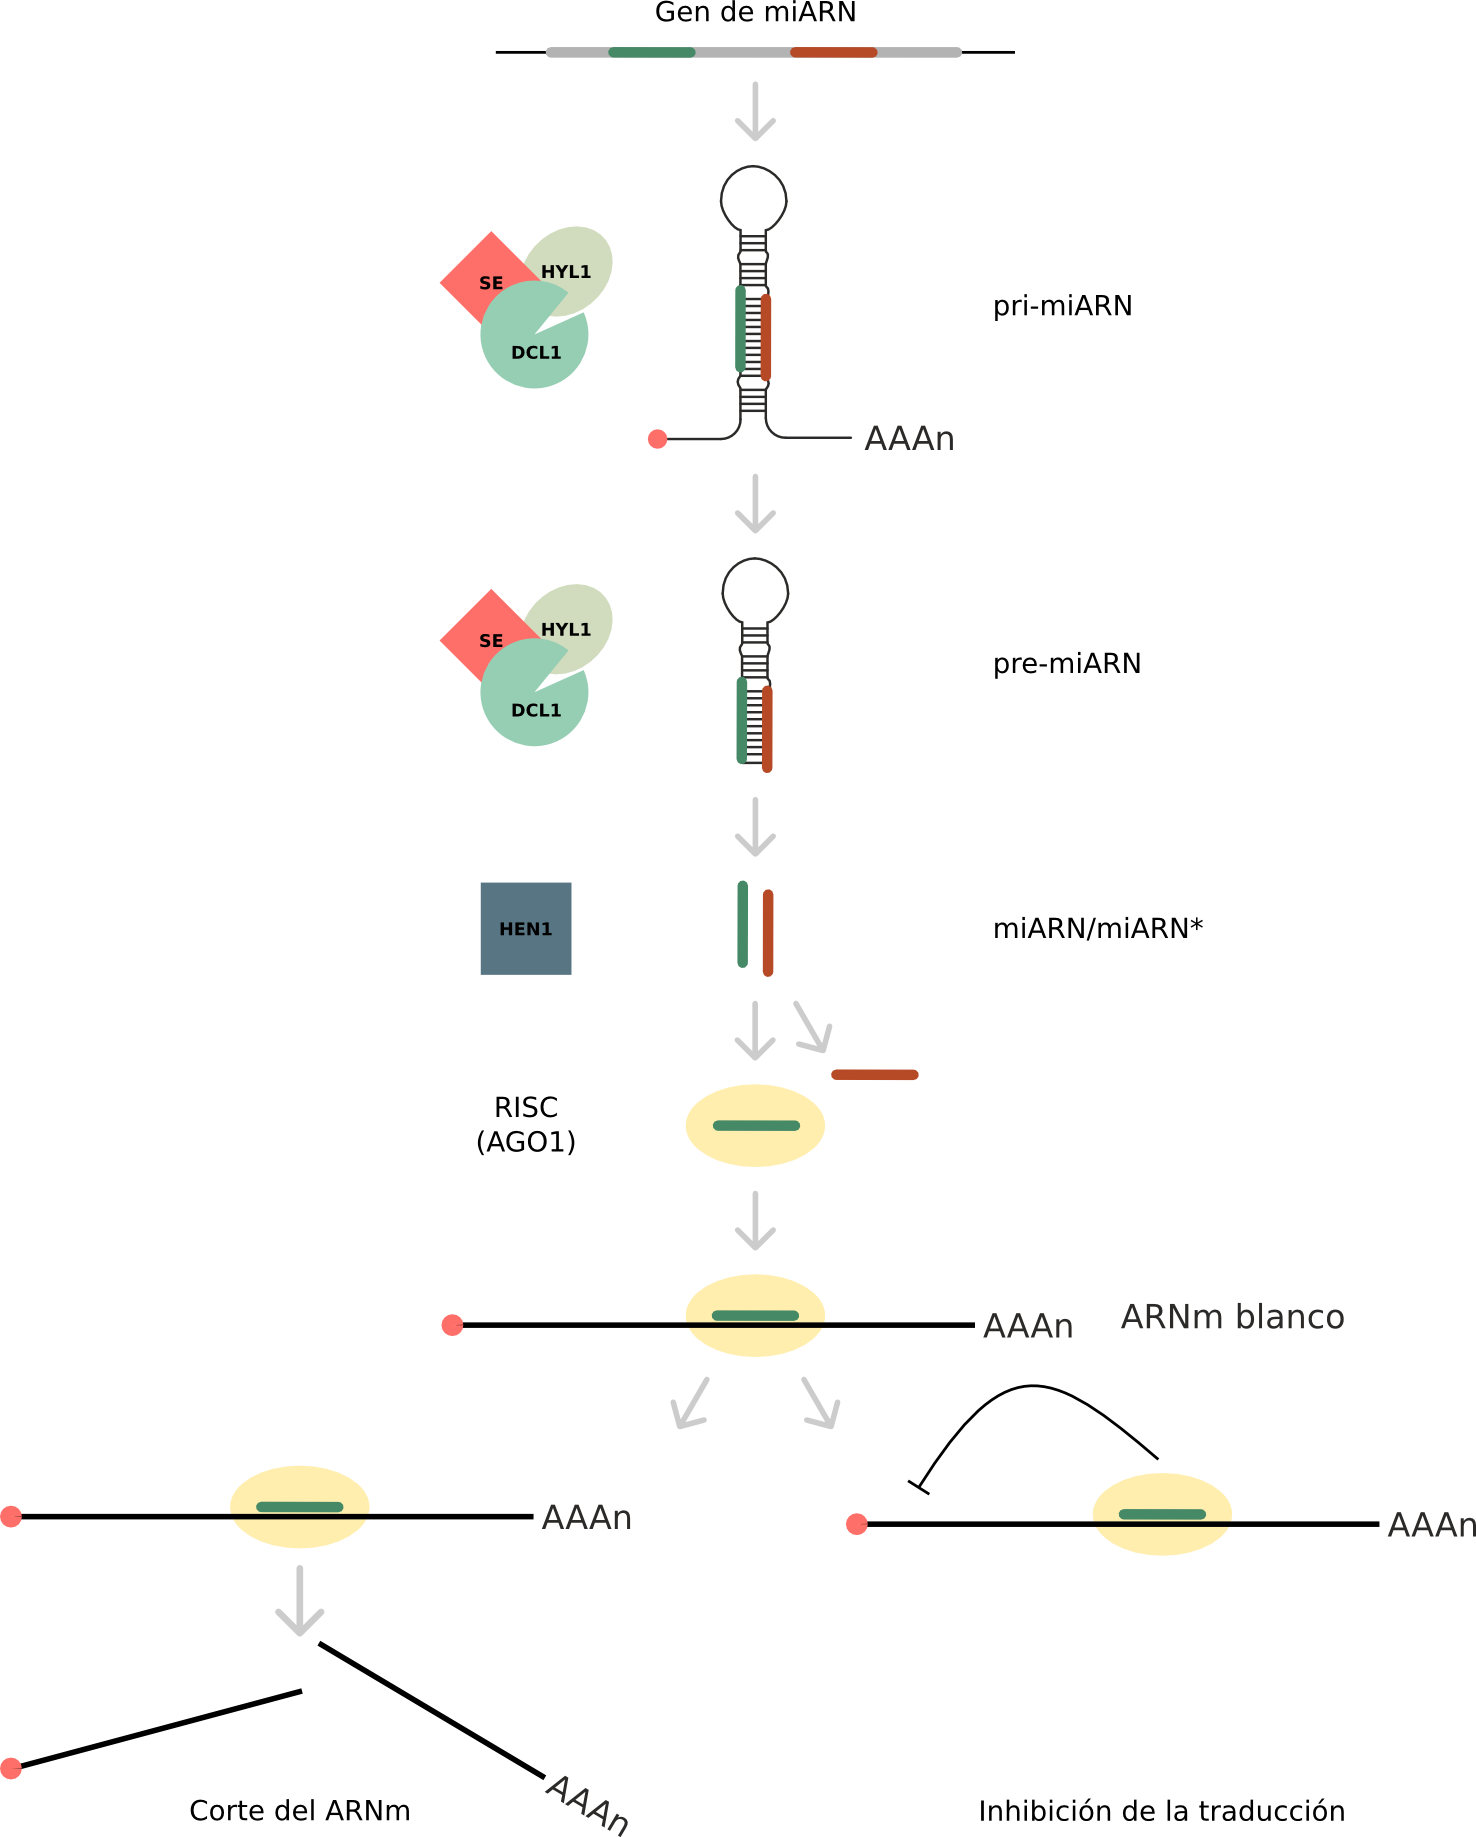
\includegraphics[width=.9\textwidth]{biogenesis_accion.png}
    \caption[Biogénesis y actividad de los miARNs en plantas]{
    \textbf{Biogenesis y actividad de miARNs en plantas.}
    Los pri-miARNs son transcriptos por la ARN polimerasa II y tienen extensa estructura secundaria en forma de tallo-burbuja (stem-loop).
    Estas estructuras son procesados en el núcleo a través de la acción de una ribonucleasa llamada DICER LIKE 1 (DCL1) en asociación con el cofactor proteico de unión a ARN de doble hebra HYPONASTIC LEAVES 1 (HYL1) y la proteína SERRATE (SE).
    El producto generado a partir de los cortes llevados a cabo por DCL1, es un dúplex miARN-miARN* que luego continúa siendo procesado por otros componentes enzimáticos hasta dar lugar al miARN maduro de 21 nt.
    Luego el miARN maduro se asocia con una proteína Argonauta (AGO), mayormente AGO1 y se incorpora dentro de un complejo de silenciamiento RISC.
    En el complejo RISC, el miARN principalmente induce el corte de los ARNm blanco, aunque algunos miARNs también regulan la expresión de sus genes blancos por represión traduccional.
    }
    \label{fig:biogenesis_accion}
\end{figure}


\section{Estructuras secundarias de precursores de miARNs}

La biogénesis de miARNs involucra el adecuado procesamiento del precursor para liberar el miARN maduro.
Para que los miARNs puedan actuar de manera correcta en la regulación de la expresión génica, es necesario que el mecanismo de biogénesis sea preciso.
Si el proceso de biogénesis no fuera preciso, cambiaría la secuencia del miARN maduro y por lo tanto el reconocimiento del sitio blanco de los ARNm por este regulado impidiendo su regulación.

Existen diferencias durante la biogénesis y mecanismo de acción entre los miARNs en plantas y en animales.
Pero además, además existen diferencias en las estructuras secundarias de los precursores de ambos reinos.
En animales, existe una marcada homogeneidad en el tamaño de los precursores de miARNs, en cambio los precursores de miARNs de plantas son muy variables en forma y tamaño (Figura \ref{fig:distribucion_precursores}). 

\begin{figure}[htbp!] 
	\centering    
	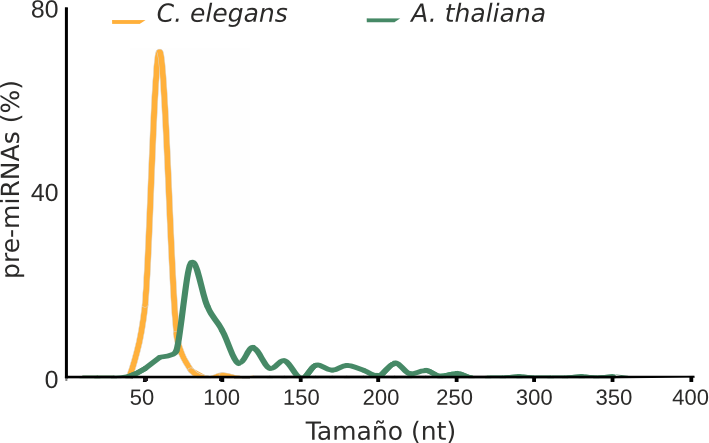
\includegraphics[width=.6\textwidth]{distribucion_precursores.png}
	\caption[Tamaños de precursores de miARNs]{
		\textbf{Tamaños de precursores de miARNs}.
		En línea naranja se muestra la distribución de tamaños de pre-miARNs en \textit{C. elegans} y en verde los pre-miARNs en \textit{A. thaliana}.
        Figura adaptada de \citep{Bologna2009}.
	}
	\label{fig:distribucion_precursores}
\end{figure}

Trabajos previos que analizaron precursores de animales señalaron que un pri-miARN típico consiste en una estructura de tallo imperfecto secundado por segmentos inestables de ARNsh en sus extremos.
El tallo imperfecto posee un tamaño de $\sim$65 nt en total que equivale a un dúplex de ARN de $\sim$33 pb  \citep{pmid16751099}
A su vez señalaron que el pri-miARN puede ser dividido en 4 partes: un loop terminal, un dúplex miARN/miARN*, un tallo inferior y secuencias flanqueantes simple hebra. 
Donde el dúplex miARN/miARN* posee una longitud de $\sim$22 pb y el tallo inferior, que se encuentra debajo de la posición donde DROSHA produce el corte, posee una longitud aproximada de $\sim$11 pb \citep{pmid16751099}.
Luego del primer corte llevado a cabo por DROSHA, el pre-miARN liberado está conformado por el dúplex miARN/miARN* y el loop terminal.

Muchos precursores en plantas tienen un tallo de $\sim$15 nt debajo del duplex miARN/miARN* seguido por un loop interno, que sirve como una señal estructural de reconocimiento por la maquinaria de procesamiento \citep{pmid17369351,pmid16751099,Mateos2010,pmid20015654} (Figura \ref{fig:ss_precursores}).
Sin embargo, este determinante de procesamiento no se encuentra en todos los precursores \citep{Mateos2010}.
Además, la biogénesis de los miARNs conservados evolutivamente como ser el miR319 y miR159 comienzan con un corte al lado del loop interno y continúa con 3 cortes adicionales en una dirección de burbuja a base hasta que finalmente el miARN es liberado \citep{Bologna2013,pmid19850910} (Figura \ref{fig:ss_precursores}).
Se ha demostrado que otros precursores de plantas liberan otros ARNs pequeños además del miARN \citep{pmid15314213,pmid20696037}, aunque los mecanismos de procesamiento subyacentes eran desconocidos.

\begin{figure}[htbp!] 
	\centering    
	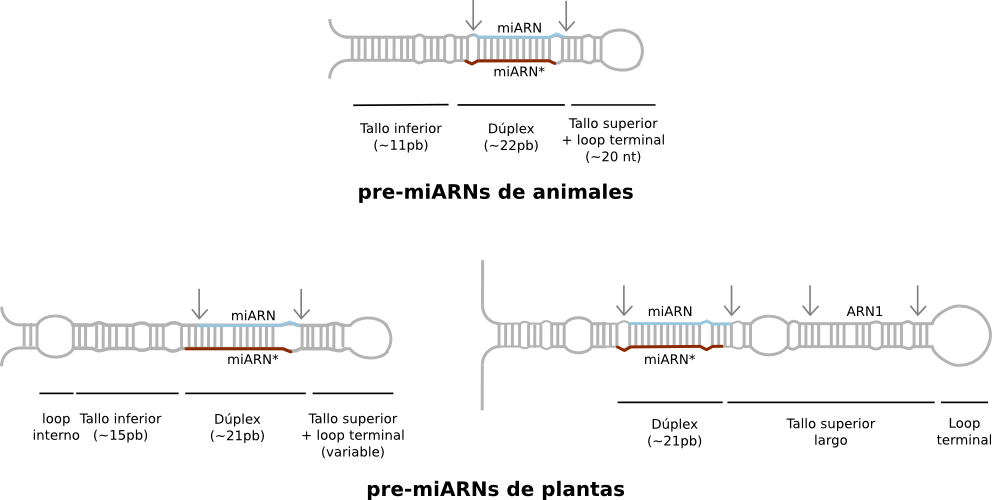
\includegraphics[width=1\textwidth]{ss_precursores.png}
	\caption[Estructuras  de precursores de miARNs]{
		\textbf{Estructuras secundarias de precursores de miARNs}.
        Arriba se muestra la estructura secundaria de precursores típicos de animales.
        Abajo a la izquierda se muestra la estructura secundaria de precursores procesados de abajo en plantas.
        Abajo a la derecha se muestra la estructura secundaria de precursores que son procesados de arriba secuenciales en plantas.
        Las flechas indican los cortes necesarios para liberar el miARN maduro.
    }
	\label{fig:ss_precursores}
\end{figure}

\section{Regulación de la expresión génica por miARNs}

\subsection{Regulación por corte del ARN blanco}

En animales existe un gran número de genes blanco mediado por miARNs y un ARNm puede estar regulado por varios miARNs, en cambio los miARNs en plantas regulan un número limitado de genes blanco \citep{Voinnet2009669}.

El ARN pequeño guía al complejo RISC hacia una molécula de ARNm complementario. 
Luego del reconocimiento de ARNm blanco por complementariedad de bases, la proteína AGO1 del complejo RISC introduce un corte en un enlace fosfodiester del ARNm.
Este corte ocurre entre las posiciones 10 y 11 desde el extremo 5' del miARN, independientemente de la longitud del miARN \citep{Mallory2004,Llave2002,pmid12931144,Xie2003,pmid15057819}.

Luego del corte mediado por el miARN, los fragmentos 3' son degradados  mediante la actividad de la enzima citoplasmática 5'-3' EXORIBONUCLEASA4 (XRN4) en En \textit{A. thaliana}  \citep{pmid15260969}
Los fragmentos 5' también pueden ser degradados por el complejo denominado Exosoma, el cual está encargado de diferentes funciones de degradación y procesamiento de ARNs \citep{pmid18160042}.
En Arabidopsis la degradación del fragmento 5', puede ser acelerada por uridilación en el extremo 3' por la enzima una enzima denomina HESO1 \citep{pmid24733911}.

\subsection{Regulación de la traducción por miARNs}

Los miARNs en animales, en general, son parcialmente complementarios a uno o más sitios presentes en la región 3' no traducida de los ARNm blancos \citep{pmid12869753,pmid8252621,Fabian} y esos ARNm raramente sufren el tipo de corte antes mencionado. 
Además, la limitada complementariedad de secuencia, permite que los miARNs de animales regulen generalmente la expresión de muchos genes blanco diferentes.
Un mecanismo que involucra la inhibición de la traducción del ARNm blanco por el miARN explica la represión de la expresión de los blancos de miARNs en animales \citep{Fabian}.
En otras ocasiones, los miARNs de animales disminuyen la vida media de los transcriptos a los que se unen \citep{pmid20703300}.
Existen algunos ejemplos de miARN de plantas también, donde se ha demostrado la existencia de un mecanismo de represión traduccional, además del corte del transcripto \citep{Schwab2005517,pmid19531599,pmid18392778,pmid18483398,pmid12893888,pmid14555699}.

\subsection{Generación de ta-siRNAs y siRNAs secundarios}
El corte de un transcripto por un miARN puede inducir la generación de ARN pequeños secundarios \citep{Allen2005207, pmid19066226,pmid19066226,pmid20643946,pmid20562854,pmid22308502}.
Existe un mecanismo por el cual se genera un ARN pequeño específico en plantas que se denomina ta-siARN (trans-acting short-interfering RNA).
Los genes que darán lugar a ta-siRNAs son transcriptos que generalmente son denominados TAS.
El transcripto es identificado y cortado por acción de un miARN que posee una secuencia complementaria al transcripto \citep{Allen2005207}.
Los fragmentos de corte de un TAS se estabilizan y por la acción de ARN polimerasas dependientes de ARN, se convierten en un ARN de doble hebra.
Luego el ARN doble hebra es procesado por una Ribonucleasa de tipo III, llamada DICER- LIKE4 (DCL4), generando ARNs pequeños de 21 nucleótidos, los ta-siARNs.
Finalmente, estos ta-siARNs se incorporan a un complejo RISC y guían el corte de los transcriptos de otros genes de manera similar a la acción de un miARN \citep{Allen2005207,pmid16040244,pmid16131612,Xie2005a}.


\section{Procesos biológicos regulados por miARNs en plantas}
Los procesos biológicos regulados por miARNs en plantas son muchos, y algunos miARNs desempeñan papeles importantes en el desarollo, otros en la trasducción de señales hormonales, respuesta a estrés y respuesta a señales del ambiente \citep{Voinnet2009669, pmid21466971, pmid19699140}.

De las 22 familias de miARNs conservados en plantas, 11 regulan factores de transcripción y la mayoría de ellos están involucrados en procesos de desarrollo o diferenciación célular \citep{Jones-Rhoades2006} (Tabla \ref{table:table_consensus}).
Por ejemplo, los genes blanco del miR172 pertenecen a la familia de factores de transcripción AP2 (APETALA2) que está involucrado en el tiempo de floración y en el desarrollo de la hoja \citep{pmid14555699, pmid12893888}.
La familia del miR319 regula factores de transcripción TCP (TEOSINTE BRANCHED1,CYCLOIDEA, PCF1/2), la familia del miR165/166 factores de transccripción HD-ZIPIII (HOMEODOMAIN-LEUCINE ZIPPER de clase III) y la familia del miR396 regulan factores de transcripción GRF (GROWTH-REGULATING FACTOR).
Todas estas familias intervienen en el desarrollo de la hoja regulando distintos factores de transcripción \citep{pmid12931144, pmid15351964, Rodriguez2010}.
El miR164, participa en el establecimiento del meristema apical del tallo, en el desarollo de la raíz y definición de los bordes de los órganos mediante la regulación de miembros de la familia de factores de transcripción NAC (NAM, ATAF1/2 and CUC2) \citep{laufus}.

Por otra parte, entre los genes blanco que no corresponden a factores de transcripción, hay genes involucrados en diversos aspectos de la biología vegetal.
Algunos codifican proteínas pertenecientes a la familia F-Box o enzimas E2 conjugantes de ubiquitina, las cuales están implicadas en la marcación de proteínas para la degradación por el proteosoma \citep{pmid19699140}.
Otros genes con función conocida codifican para proteínas involucradas en la transducción de señales hormonales, o proteínas involucradas en el metabolismo energético, la respuesta a estrés o déficit de nutrientes.

Por otro lado, en especies en las que se han realizados estudios de ARN pequeños por técnicas de secuenciación de alto rendimiento, se han encontrado miARNs no conservados \citep{citeulike:8816489, Rodriguez2010, Rajagopalan2006}.
Los genes blanco regulados por estos miARNs tienen funciones más variables que los blanco de los miARNs conservados, no esta clara la importancia biológica de estas interacciones \citep{citeulike:8816489}.

En esta tesis nos enfocaremos principalmente en las familias de miARNs conservadas entre distintas especies de plantas (Tabla \ref{table:table_consensus}).
Estas familias han sido estudiadas profundamente, por lo que su mayoría se encuentran ampliamente caracterizadas.


\section{Predicción de genes blanco de miARNs}

\subsection{Interacción de miARN-ARNm blanco}

Los miARNs reconocen secuencias complementarias en ARNm blancos provocando su corte o el arresto traduccional.
Originalmente, se creía que los miARNs de plantas tenían complementariedad casi perfecta con los genes blanco regulados por ellos \citep{pmid19167326,pmid12869753,pmid12242443}.
Sin embargo, en artículos más recientes se ha demostrado que existen genes blanco regulados por miARNs de distintas especies, con un un mayor número de "mismatches" a lo que se creía previamente \citep{German2008} e incluso con interacciones no canónicas como "bulges" de varios nucleótidos \citep{pmid24561804} (Figura \ref{fig:interaccion_miRNA_target}).
Esto hace que la predicción de genes blanco regulados por miARNs en plantas no sea trivial y que se necesite información extra además de la interacción del par miARN-blanco.

Por otro lado en animales, la especificidad y la función de los miARNs están determinados por los nucleótidos 2 a 7 de la parte 5' del miARN maduro (llamada región "semilla" del miARN) \citep{pmid12672692}.
Dichos nucleótidos deben ser complementarios al ARNm blanco (Figura \ref{fig:interaccion_miRNA_target}).

\begin{figure}[htbp!] 
	\centering    
	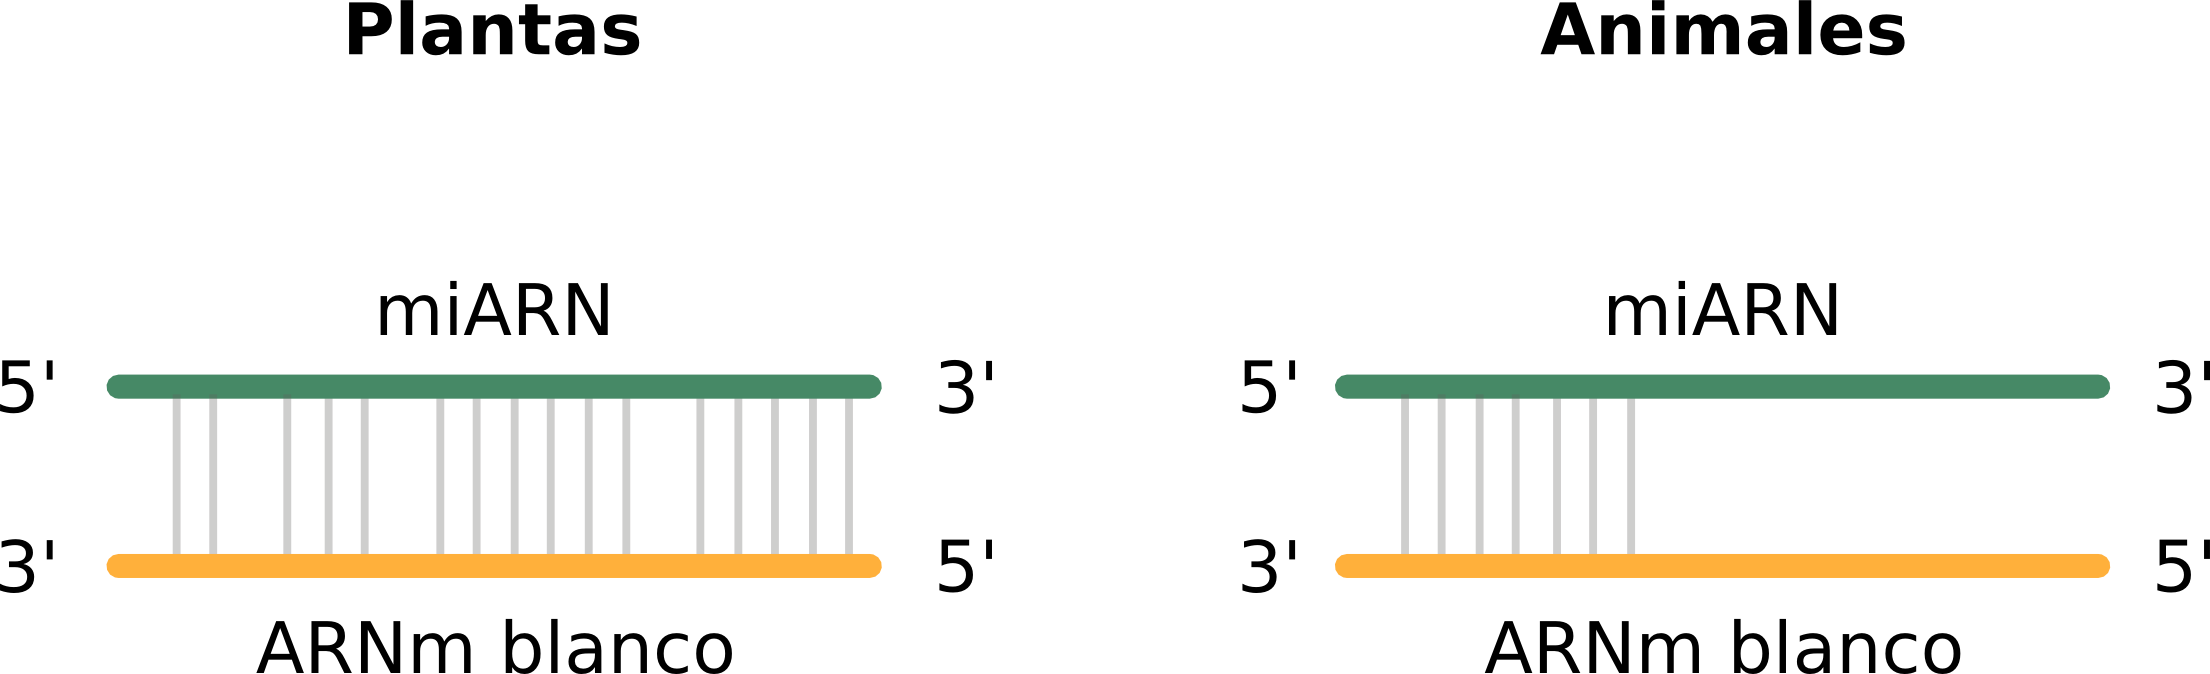
\includegraphics[width=.7\textwidth]{interaccion_miRNA_target.png}
	\caption[Interacción de miARN-ARNm blanco]{
		\textbf{Interacción de miARN-ARNm blanco.}
        A la izquierda se muestra una interacción del par miARN-ARNm blanco en plantas.
        A la derecha se muestra una interacción del par miARN-ARNm blanco en animales.
        Las líneas verticales grises representan bases apareadas, la ausencia de líneas puede ser "mismatches" o "bules".
	}
	\label{fig:interaccion_miRNA_target}
\end{figure}


\subsection{Métodos para predicción de genes blanco de miARNs en animales}
Existen muchos métodos para la predicción de genes blanco de miARNs que fueron desarrollados por distintos grupos de investigación.
Gran parte de ellos continúan manteniendo y actualizando sus algoritmos. El grupo de Cohen en el EMBL propuso el primer predictor de genes blanco de miARNs en 2003 \citep{pmid14691535} que luego fue actualizado en el 2005 \citep{pmid16337999}.
TargetScan y TargetScanS fueron desarrollados por Bartel en el MIT y Burge en Cambridge \citep{pmid18955434,pmid17612493,pmid14697198,pmid15652477}.
DIANA-microT, otra herramienta popular que fue creada por el grupo de Hatzigeorgiou, fue actualizada recientemente a la versión 5.0 \citep{pmid19765283,pmid21551220,pmid23680784}.
El grupo de Rajewsky publicó su predictor de genes blanco en el 2005 y fue actualizado en el 2011 \citep{pmid15383676,pmid22086949}. 

Hay dos categorías de modelos predictivos: heurísticos y empíricos.
Los modelos heurísticos utilizan algoritmos de detección que buscan posiciones a lo largo de la secuencia del ARNm y funciones de puntajes que filtran los blanco mediante la combinación de varios valores de entrada.
Los primeros predictores aplican enfoques heurísticos, debido a la falta de una cantidad suficiente de datos para construir los modelos basados en el conocimiento empírico.

Los modelos predictivos utilizan entradas que se derivan del conocimiento de los detalles mecanísticos de las interacciones miARN-ARNm.
La entrada  más utilizada de los modelos predictivos, es la complementariedad de base entre el miARN y ARNm.
Los miARNs de animales por lo general se unen al ARNm con sólo algunas posiciones que están apareadas \citep{pmid15345038}, pero la complementariedad del apareamiento de bases en la región semilla (seed), que comprende los ocho primeros nucleótidos en el extremo 5' del miARN, es particularmente importante.
Los parámetros de entradas de accesibilidad del sitio y de conservación evolutiva se utilizan para aumentar la especificidad.
La mayoría de los predictores usan software existentes, como el Vienna RNA package \citep{pmid22115189}, mFold \citep{pmid12824337}, DINAMelt \citep{pmid15980540} y mFold \citep{pmid15215366}, para el cálculo de la energía libre.
El uso de la conservación evolutiva de los genes blanco de miARNs está motivada por la premisa de que las especies 'similares' deben compartir miARNs comunes y genes blanco comunes.
Sin embargo, esto conduce a la omisión de los genes blanco no conservados \citep{pmid17254305, pmid21674004}.


\subsection{Métodos para predicción de genes blanco de miARNs en plantas}
Los algoritmos mencionados anteriormente son utilizados generalmente para predecir genes blanco de miARNs en animales.
Algunos de ellos, como MiRanda, se utilizan tanto en animales como en plantas.
Existen herramientas diseñadas específicamente para la predicción de genes blanco de miARNs en plantas.
Algunas de ellas fueron implementadas como herramientas independientes, otras como serivdores web y algunas como ambos.

La herramienta psRNATarget \citep{pmid21622958} utiliza un enfoque de programación dinámica, alineando las secuencias utilizando el algoritmo de Smith-Waterman modificado y aplicando el algoritmo 'RNAup'.
Targetfinder \citep{pmid15598838} implementa un programa "FASTA" junto con un sistema de puntuación para "mismatches", "bulges" o "gaps" para alinear las secuencias.
TAPIR \citep{pmid20430753} está integrado con dos opciones de búsqueda, el motor de búsqueda "FASTA" (para búsquedas rápidas), y el motor de búsqueda "RNA hybrid" (para obtener resultados precisos).
La herramienta Target-align \citep{pmid20934992} también emplea el método de puntuación basado en el algoritmo de Smith-Waterman para predecir las complementariedades entre los miARNs y los RNAs mensajeros.
Por último, la herramienta p-TAREF \citep{pmid22206472} implementa un modelo de regresión de máquinas de vectores de soporte (SVR en ingés "support vector regression") y utiliza la información de la "variación de la densidad de dinucleótido" alrededor del sitio blanco de un conjunto de datos de \textit{A. thaliana}, \textit{Oryza sativa}, \textit{Medicago truncatula} y \textit{Solanum lycopersicum}.

Además existen otras herramientas que son utilizadas para predecir genes blanco de miARNs pero que no fueron específicamente diseñadas para esto.
Por ejemplo, la herramienta  Web miRNA designer, WMD3 \citep{pmid18269576} es utilizada para el diseño del miARNs artificiales para silenciar la expresión de genes blanco específicos.
Pero esta herramienta también es empleada para la predicción de genes blanco de miARNs en plantas.
RNAHybrid \citep{Kruger01072006} es una herramienta utilizada para buscar la energía mínima libre de un ARN largo y uno corto.
La secuencia corta se hibrida con la parte más adecuada de la secuencia larga.
La herramienta está destinada principalmente para la predicción de genes blanco de miARNs, pero no es su único uso.

Patmatch \citep{Yan01072005} que está integrado en "The Arabidopsis Information Resource" (TAIR)\footnote{https://arabidopsis.org} permite realizar búsqueda de secuencias de nucleótidos o de péptidos corto, como dominios pequeños o motivos.
Esta herramienta puede ser adaptada, para utilizarla como herramienta de búsqueda de genes blanco de miARNs en plantas.

La mayoría de las herramientas específicas de plantas fueron desarrolladas para predecir genes blanco con una alta especificidad en el organismo modelo \textit{A. thaliana}, si se utilizan los parámetros de predicciones óptimos.
Y los sistemas de puntajes optimizados de Arabidopsis no se pueden utilizar como un umbral en el análisis de organismos no modelos \citep{pmid24885295}.
Además estas herramientas en general detectan una gran cantidad de potenciales genes blanco (que incluyen los validados experimentalmente), pero su debilidad radica en que predicen una gran número de falsos positivos.

\subsection{Identificación de genes blanco regulados por miARNs mediante técnicas de secuenciación de alto rendimiento}
Con los avances de los métodos de secuenciación de alto rendimiento o "next-generation sequencing", la identificación sistemática de genes blanco de miARNs específicos en un tiempo corto ya es un hecho.
Un método denominado PARE (Construction of Parallel Analysis of RNA Ends) \citep{pmid19247285}.
La misma consiste en una combinación de la estrategia modificada 5´RACE, en donde se secuencian masivamente ARNs que carecen de 5’ CAP.
Esto implica que se detectan ARNm fragmentados, pero no los intactos.
Además, el proceso de secuenciación permite identificar el sitio exacto de fragmentación o corte del ARNm.
Por este motivo se suele referir a las bibliotecas PARE como el degradoma del ARN de las células. 

Un elemento importante es que los miARNs y siARNs guían el corte de sus ARNm blanco entre las posiciones 10-11 del extremo 5' del ARN pequeño.
Es decir, dada una interacción miARN/sitio blanco, uno puede predecir exactamente donde se producirá el corte del ARNm.
Y si este corte realmente existe en las células, los fragmentos de ARNm detectados por PARE deberían estar enriquecidos en este lugar preciso del ARNm.

A partir de las bibliotecas de PARE, se han desarrollado diferentes herramientas como SeqTar \citep{pmid22140118}, que es un método para la identificación de corte guíado por miARNs de degradoma de transcriptos de plantas.
Por otro lado, CleaveLand \citep{pmid19017659} es un pipeline computacional para la detección de cortes de miARNs en datos de degradoma.
Esta herramienta toma como entrada secuencias de degradoma, ARNs pequeños y una base de datos de ARNm y devuelve los potenciales genes blanco de esos ARNs pequeños. 
sPARTA (small RNA-PARE target analyzer) \citep{pmid25120269} es un pipeline paralelizado, para el análisis integrado de miARNs en plantas y un conjunto de ARNm.
Este pipeline incluye un software de identificación de nuevos genes blanco regulados por miARNs y utiliza datos de PARE.

Por otro lado, la herramienta PAREsnip permite realizar búsqueda de potenciales genes blanco de todos los ARN pequeños obtenidos de técnicas de secuenciación de alto rendimiento.
Mediante la búsqueda de genes blanco de todo el "sRNAome" se pude facilitar identificación de genes blanco de ARN pequeños a grande escala.

